\documentclass[aspectratio=169]{beamer}

\usepackage{../theme/polygl0ts}

%%%%%%%%%%%%%%%%%%%%%%%%%%%%%%%%%%%%%%%%%%%%%%%%%%%%%%%%%%%%%%%%%%%%%%%%%%%%%%%
% Title Setup
%%%%%%%%%%%%%%%%%%%%%%%%%%%%%%%%%%%%%%%%%%%%%%%%%%%%%%%%%%%%%%%%%%%%%%%%%%%%%%%
\title{Lesson 0: What is CTF and who is flagbot?}
\subtitle{}
\author{Leonardo Galli}
\date{23. September 2019} 
 
\begin{document} 

\titleframe

\tocframe

\section{Introduction to CTFs}
 
\begin{frame}[fragile]
\frametitle{What is CTF?}
\begin{itemize}
    \item Stands for Capture the Flag
    \item Sport consisting of solving hacking challenges
    \item Usually done in a team
    \item Flag as proof of solving a challenge
    \begin{itemize}
        \item Example flag: \inlinecode[python]{flagbot{sh0uld_h4ve_g0ne_f0r_the_he4d}}
    \end{itemize}
    \item Challenges grouped into five major categories: pwn, reversing, web, crypto and misc
\end{itemize}
\end{frame}

\subsection{The Different Categories}

\begin{frame}
    \frametitle{pwn challenges}
    \begin{columns}
        \column{0.5\textwidth}
            \centering
            \begin{itemize}
                \item Usually a small application
                \item Get remote code execution by finding a vulnerability
                \item Often need to use a disassembler / decompiler
            \end{itemize}
        \column{0.5\textwidth}
            \centering
            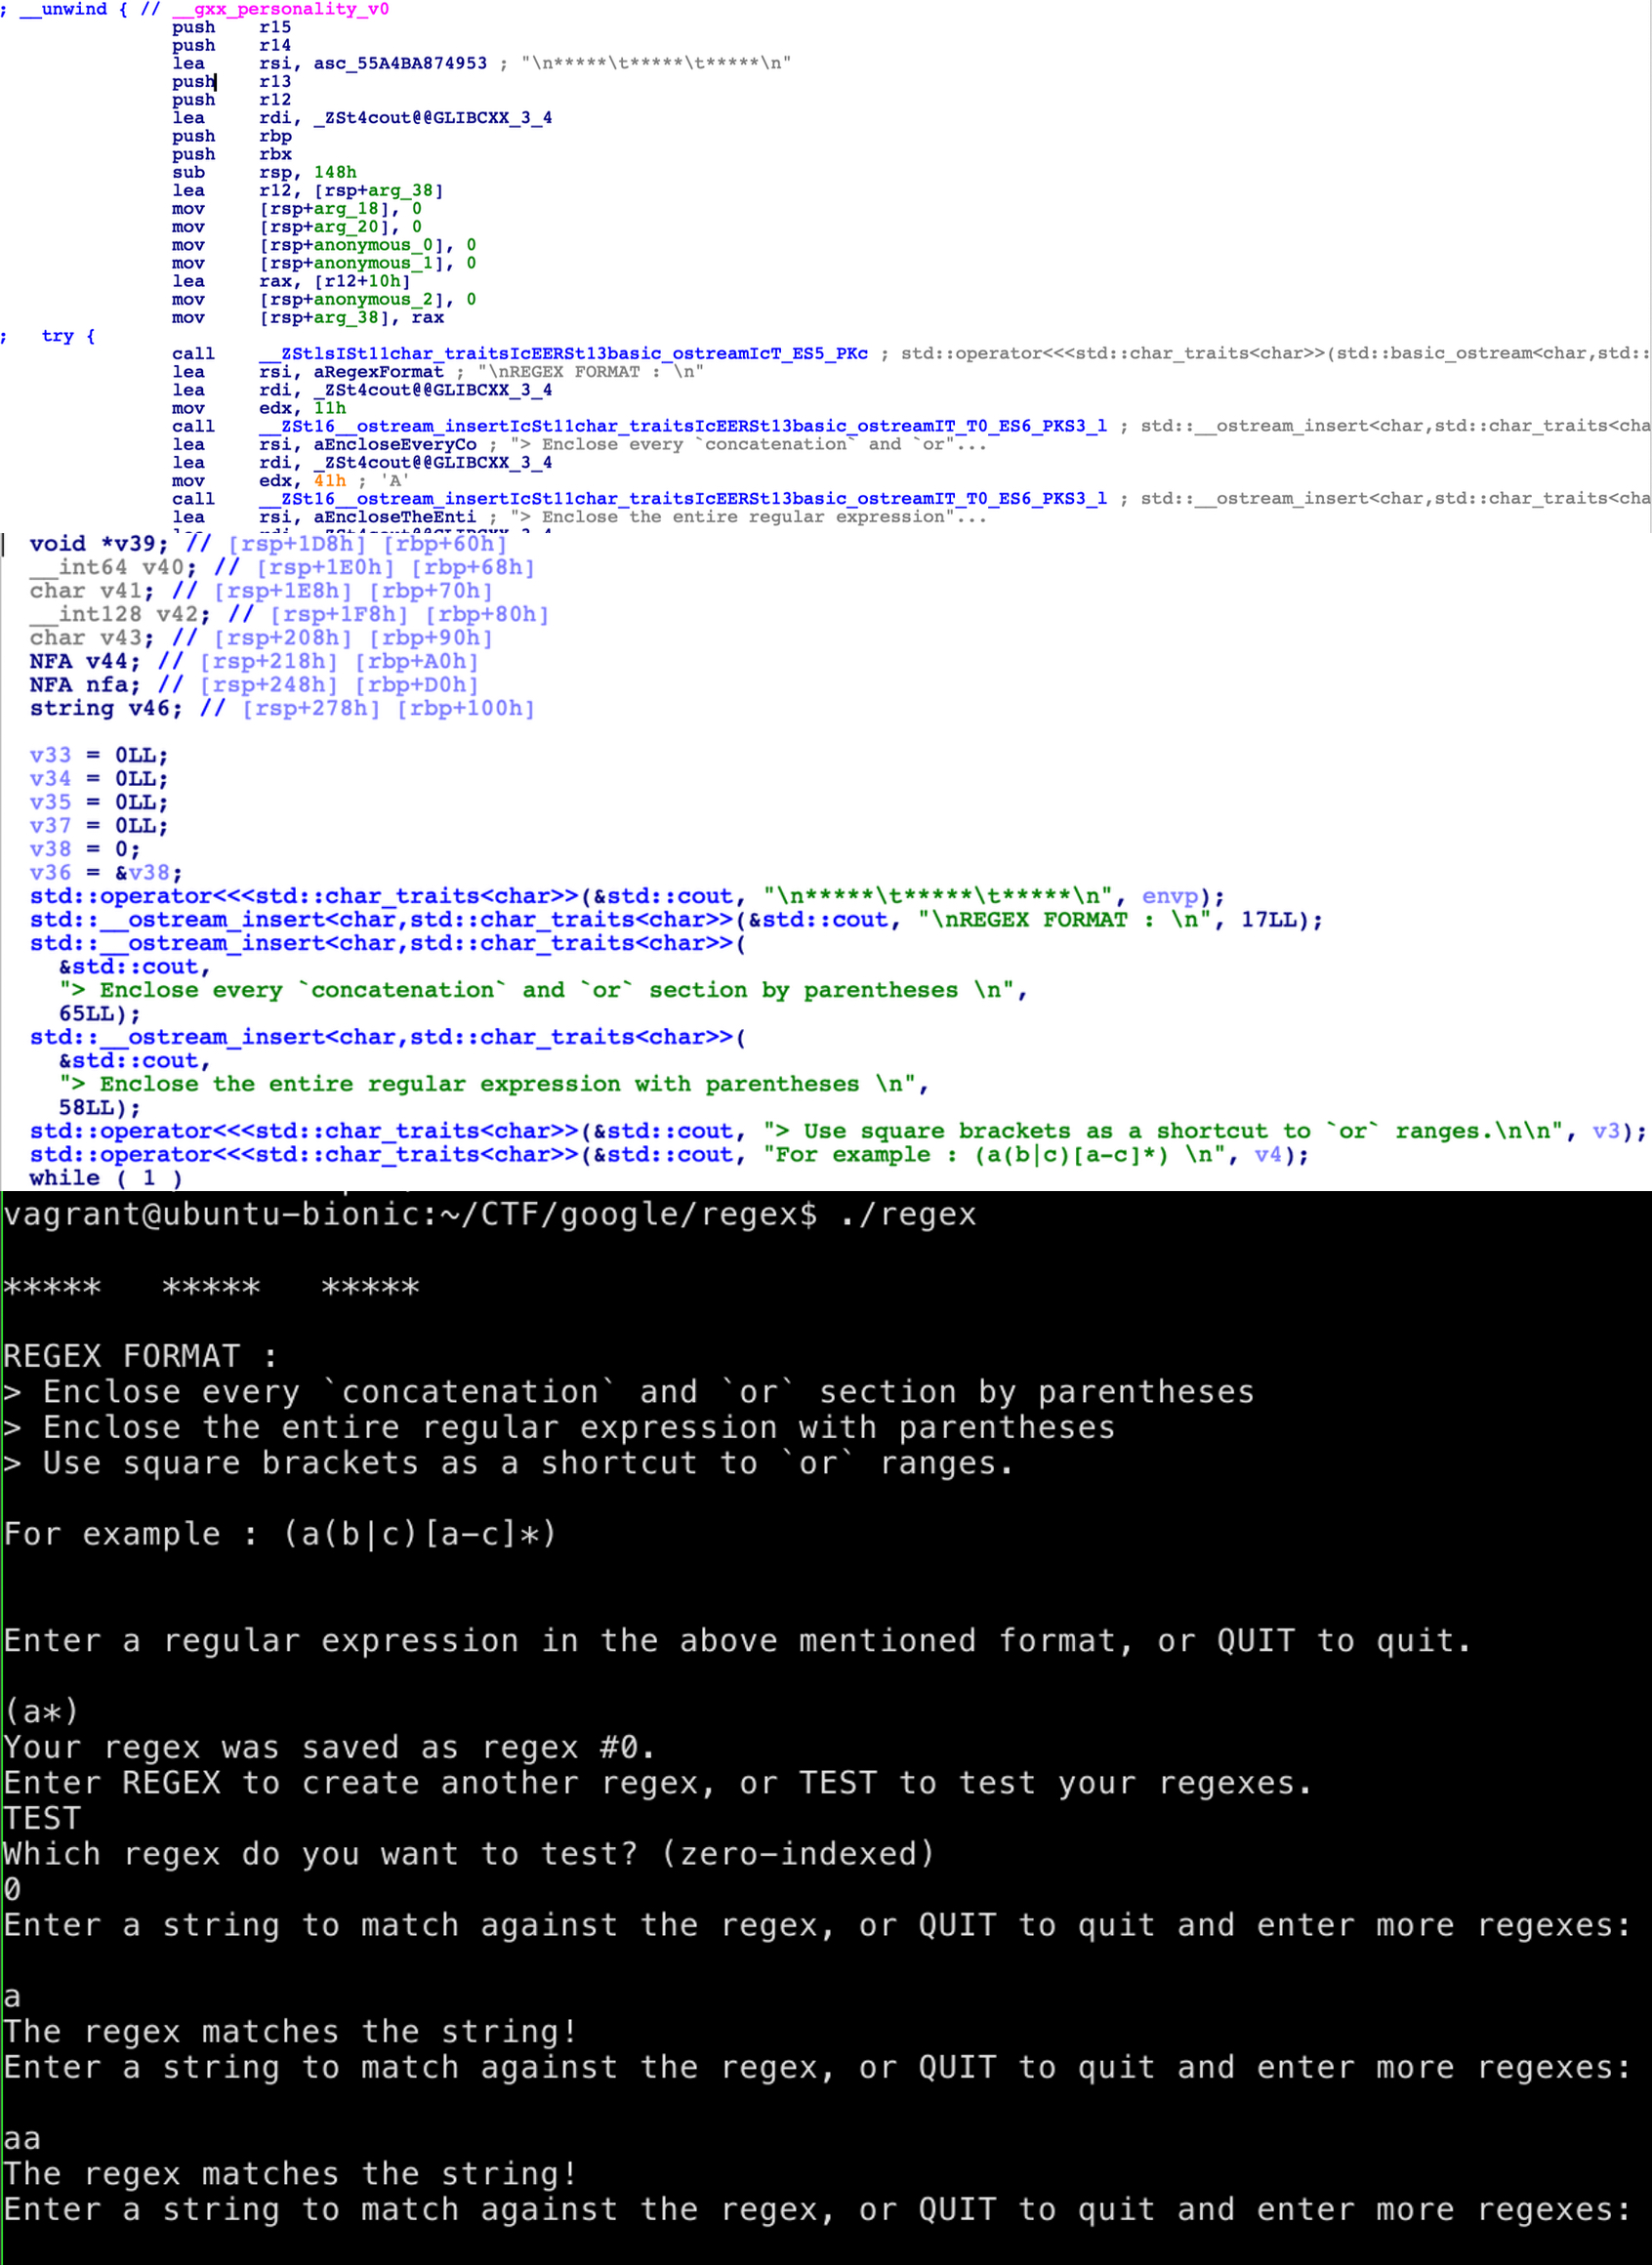
\includegraphics[width=\textwidth]{pwn_example.jpg}
    \end{columns}
\end{frame}

\begin{frame}
    \frametitle{reversing challenges}
    \begin{columns}
        \column{0.5\textwidth}
            \centering
            \begin{itemize}
                \item Very similar to pwn challenges
                \item Figure out, what the program {\textbf{exactly}} does
                \item Examples are:
                \begin{itemize}
                    \item Key generator
                    \item Heavily obfuscated binary
                \end{itemize}
            \end{itemize}
        \column{0.5\textwidth}
            \centering
            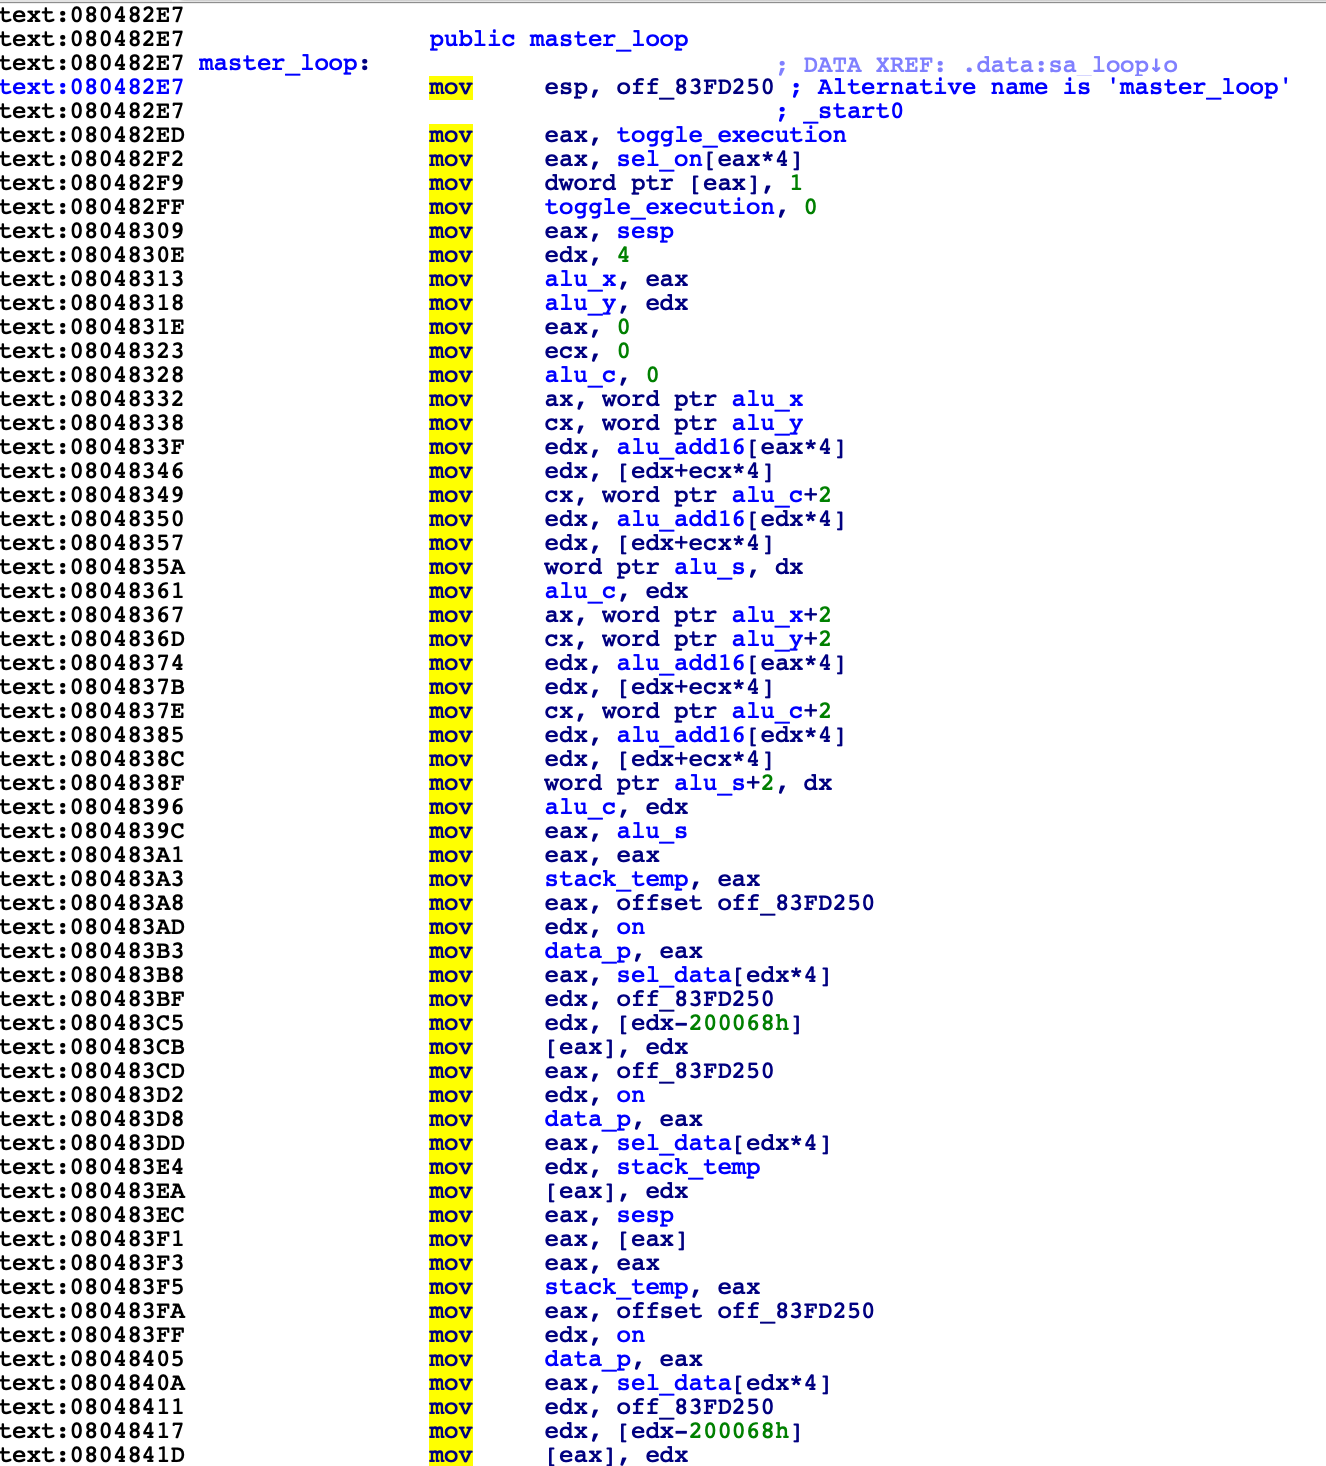
\includegraphics[width=\textwidth]{reversing_example.png}
    \end{columns}
\end{frame}

\begin{frame}
    \frametitle{web challenges}
    \begin{itemize}
        \item Focuses on web services, languages and frameworks
        \item Often a ``blackbox''
        \item Could even have to exploit language bugs
        \item Examples are:
        \begin{itemize}
            \item SQL Injection
            \item XSS
            \item Badly implemented authentication
        \end{itemize}
    \end{itemize}
\end{frame}

\begin{frame}
    \frametitle{crypto challenges}
    \begin{itemize}
        \item Short for cryptography
        \item Find weaknesses in specific implementation of existing cryptography protocol
        \item Analyze published research for specific cryptography protocol
        \item Examples are:
        \begin{itemize}
            \item Using $3$ as the exponent in RSA
            \item Not initializing the IV
        \end{itemize}
    \end{itemize}
\end{frame}

\begin{frame}
    \frametitle{misc challenges}
    \begin{columns}
        \begin{column}{0.5\textwidth}
            \begin{itemize}
                \item No real focus
                \item Often includes steganography and some cryptography
                \item Examples are:
                \begin{itemize}
                    \item Hidden data inside an image
                    \item Scavenger hunt
                    \item Reading unknown symbols
                \end{itemize}
            \end{itemize}
        \end{column}
        \begin{column}{0.5\textwidth}
            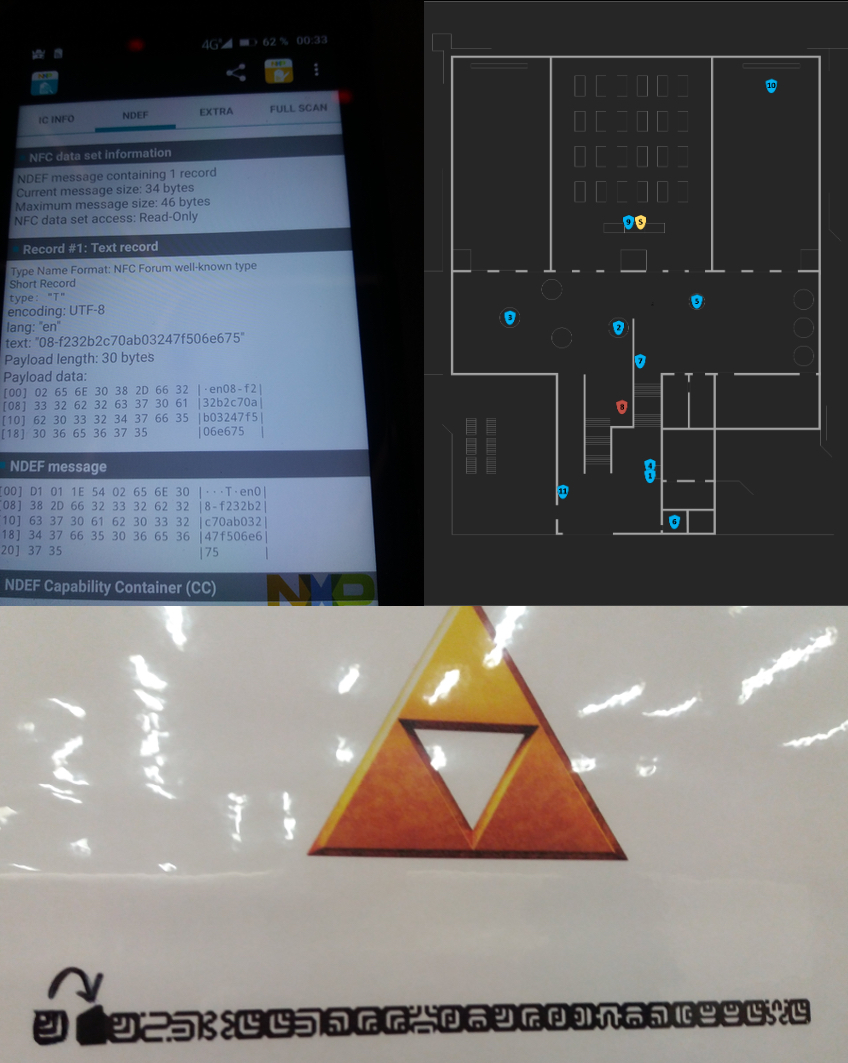
\includegraphics[width=\textwidth]{misc_example.jpg}
        \end{column}
    \end{columns}
\end{frame}

\section{About Us}

\begin{frame}
    \frametitle{Who is flagbot?}
    \begin{itemize}
        \item We are a VIS committee
        \item Meet every Monday for Training
        \item Participate in cool CTF events over the Weekends
        \item Currently ranked \#1 in Switzerland and \#109 overall on CTFtime
        \item In the process of growing our team as well as infrastructure
    \end{itemize}
\end{frame}

\begin{frame}
    \frametitle{ctf@vis.ethz.ch Mailing list}
    \begin{itemize}
        \item Subscribe at \href{https://lists.vis.ethz.ch/postorius/lists/ctf.lists.vis.ethz.ch/}{https://lists.vis.ethz.ch/postorius/lists/ctf.lists.vis.ethz.ch/}
        \item We will send E-Mails there, whenever we participate in a CTF event
        \item Can be used to ask questions, but please keep them \textbf{spoiler free!}
        \item In general used for announcements
    \end{itemize}
\end{frame}

\section{Practical Examples}

\begin{frame}
    \frametitle{Two example exploits}
    \begin{itemize}
        \item Babyrop
        \begin{itemize}
            \item My first exploit
            \item Very simple challenge
        \end{itemize}
        \item Nuts
        \begin{itemize}
            \item One of my latest exploits
            \item Exploits a Kernel built by one of our team members
        \end{itemize}
    \end{itemize}
\end{frame}

\section{What to do?}

\begin{frame}
    \frametitle{picoCTF}
    \begin{itemize}
        \item Beginner CTF
        \item Ideal way to introduce people to CTF
        \item Register here: \href{https://2018game.picoctf.com}{2018game.picoctf.com}
    \end{itemize}
\end{frame}

\begin{frame}
    \frametitle{picoCTF recommended challenges}
    \begin{columns}[T]
        \begin{column}{0.5\textwidth}
            Beginner
            \begin{itemize}
                \item Reversing Warmup 1
                \item grep 1
                \item net cat
                \item grep 2
            \end{itemize}
        \end{column}
        \begin{column}{0.5\textwidth}
            Intermediate
            \begin{itemize}
                \item assembly-0
                \item assembly-1
                \item Buffer overflow 0
                \item leak-me
            \end{itemize}
        \end{column}
    \end{columns}
    \vfill
    \begin{columns}[T]
        \begin{column}{0.5\textwidth}
            Advanced
            \begin{itemize}
                \item be-quick-or-be-dead-1
                \item Buffer overflow 1
                \item Buffer overflow 2
            \end{itemize}
        \end{column}
        \begin{column}{0.5\textwidth}
            Expert
            \begin{itemize}
                \item got-2-learn-libc
                \item echooo
                \item got-shell?
            \end{itemize}
        \end{column}
    \end{columns}
\end{frame}

\end{document}